\documentclass[11pt,a4paper]{article}

\usepackage{graphicx}
\usepackage[prologue]{xcolor}
\usepackage{amsmath}
\usepackage{amssymb}
\usepackage{tabularx}
\usepackage{booktabs}
\usepackage{tikz}
\usetikzlibrary{decorations.pathreplacing}
\usepackage{hyperref}
\usepackage[nameinlink]{cleveref}
\definecolor[named]{ACMBlue}{cmyk}{1,0.1,0,0.1}
\definecolor[named]{ACMYellow}{cmyk}{0,0.16,1,0}
\definecolor[named]{ACMOrange}{cmyk}{0,0.42,1,0.01}
\definecolor[named]{ACMRed}{cmyk}{0,0.90,0.86,0}
\definecolor[named]{ACMLightBlue}{cmyk}{0.49,0.01,0,0}
\definecolor[named]{ACMGreen}{cmyk}{0.20,0,1,0.19}
\definecolor[named]{ACMPurple}{cmyk}{0.55,1,0,0.15}
\definecolor[named]{ACMDarkBlue}{cmyk}{1,0.58,0,0.21}
\hypersetup{colorlinks,
  linkcolor=ACMOrange,
  citecolor=ACMPurple,
  urlcolor=ACMDarkBlue,
  filecolor=ACMDarkBlue}

\title{COMP4031: Scientific Computing coursework}
\author{Lawrence Mitchell\thanks{\texttt{lawrence.mitchell@durham.ac.uk}}}
\date{October 2019}
\renewcommand{\vec}[1]{\ensuremath{\mathbf{#1}}}
\begin{document}

\maketitle{}

\noindent
This assignment is to be completed and handed in via DUO. You should
submit a Jupyter notebook containing both your code (which should be
runnable), and a discussion of your implementation choices and
observations and answers to the questions. You can use any of the code
presented in the lectures, appropriately attributed.

\section{The convection-diffusion equation}
\label{sec:part1}

We will simulate a very simple model of heat transfer driven by a
``wind''. We will do so in a 2D vertical slice of the atmosphere.
We'll use $T(x, y; t)$ to describe the temperature field, and impose a
background wind field shown in \cref{fig:wind}
\begin{equation}
  \label{eq:2}
  \vec{w} = \begin{bmatrix}v_0\\v_1\end{bmatrix} = \begin{bmatrix}
    4 \sin 2\pi y \cos \frac{\pi x}{2}\\
    -\sin \frac{\pi x}{2} \cos 2\pi y\end{bmatrix}.
\end{equation}
\begin{figure}[htbp]
  \centering
  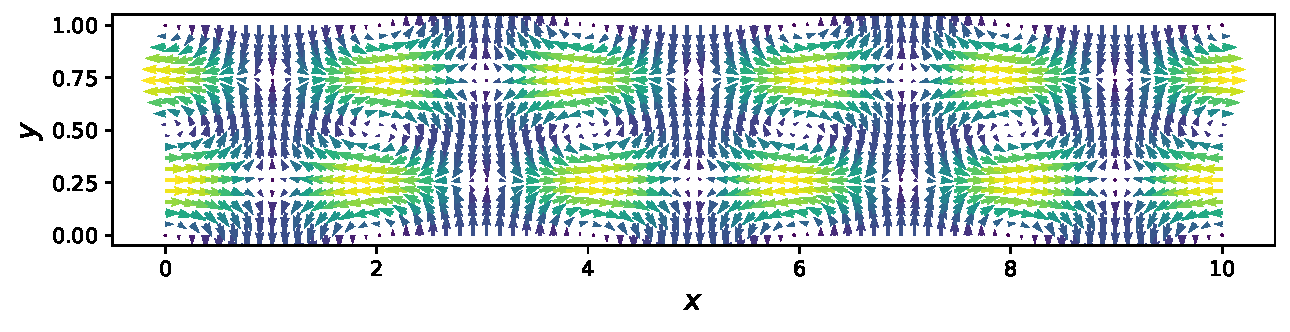
\includegraphics[width=0.8\textwidth]{wind-field}
  \caption{Background wind field of \cref{eq:2}}
  \label{fig:wind}
\end{figure}

The relevant equation describing the time evolution of the temperature
field is to find $T$ satisfying
\begin{equation}
  \label{eq:1}
  \begin{aligned}
  \partial_t T - \nu \nabla^2 T + \nabla \cdot (\vec{w} T) &= 0 &&\text{ in } \Omega\\
  T &= 1 - y &&\text{ on } \partial\Omega
  \end{aligned}
\end{equation}
where $\nu > 0$ is a scalar constant controlling the relative
importance of the convective and diffusive terms. To begin, we will
set $\nu = 1$. We have carefully arranged that the wind $\vec{w}$ is
has zero divergence, we can therefore rewrite the convective term as
\begin{equation}
  \label{eq:3}
  \vec{w} \cdot \nabla T
\end{equation}
which simplifies the implementation somewhat.

We will discretise this problem on the rectangular domain $\Omega =
[0, 10] \times [0, 1]$. As shown in \cref{fig:omega}
\begin{figure}[htbp]
  \centering
  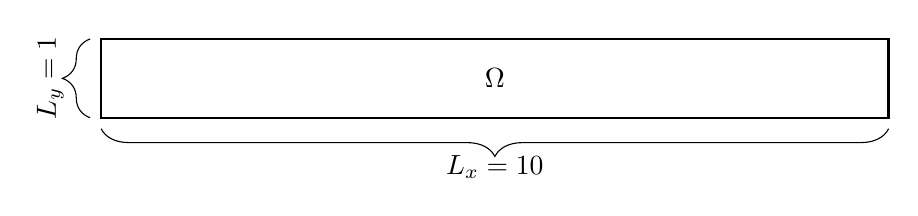
\begin{tikzpicture}
    \draw[thick, black] (0,0) rectangle node{$\Omega$} (10, 1);
    \draw [decorate,decoration={brace, amplitude=10pt, mirror, raise=4pt}]
    (0,0) -- (10,0) node [black,midway,below, yshift=-10pt] {$L_x = 10$};

    \draw[decorate,decoration={brace, amplitude=10pt, raise=4pt}]
    (0,0) -- (0, 1) node [rotate=90,black,midway, above, yshift=10pt] {$L_y = 1$};
  \end{tikzpicture}
  \caption{Simulation domain}
  \label{fig:omega}
\end{figure}


We will discretise this equation in two stages, first discretising in
space, and then in time. We will use explicit timestepping, but you
will be programming more than one such scheme, so you may find it
helpful to structure your program to discretise the spatial term
independently from the time derivative.

As a first step, we will use explicit Euler for the time derivative.
Derive a finite difference discretisation for the spatial terms. You
should use an appropriate centred difference scheme for the Laplacian
term. For the first derivative, as we saw in class, we should use a
one-sided derivative. There are a number of options here:
\begin{itemize}
\item left neighbour;
\item right neighbour;
\item adaptive ``upwinding'' based on the value of the wind.
\end{itemize}
Implement the timestepping scheme and spatial derivatives. Discuss
whether you observe any differences in the accuracy and/or numerical
stability of the solution scheme with the different choices for the
$\nabla T$ term.

This section is worth 30/100 marks. Marks are provided for
correctness (10), elegant/simple code (10), and the discussion of the
choice of derivative approximations (10).

\section{Numerical experiments, better time-stepping}
\label{sec:part2}

Implement a higher-order explicit RK scheme as well as explicit Euler.
Justify your choice based on the order of your spatial discretisation.

Fix the final time at $t = 1$. Discuss answers to the following
questions:

\begin{itemize}
\item For the two time-stepping schemes, how does time to solution
  change as you increase the resolution?
\item What observations can you make about the required timestep size
  as you increase the resolution?
\item Experiment with smaller values of $\nu$, does this have any
  impact on the stability of your solution?
\end{itemize}

This section is worth 30/100 marks. Marks are provided for
correctness of the RK implementation, and the discussion in your
answers to the questions.

\section{Stationary states, implicit time-stepping}
\label{sec:part3}
As long as $\nu > 0$, this equation has a steady state. We can find it
by setting the time derivative to zero, and solving the resulting
stationary equation
\begin{equation}
  \label{eq:4}
  \begin{aligned}
  -\nu \nabla^2 T + \vec{w} \cdot \nabla T &= 0 &\text{ in } \Omega\\
  T &= 1 - y &\text{ on } \partial\Omega.
  \end{aligned}
\end{equation}
To do this, we will discretise the operator and assemble it into a
matrix. The solution for $T$ can then be obtained by solving the
matrix equation
\begin{equation}
  \label{eq:5}
  A T = F,
\end{equation}
where $A$ is the discretised operator, $T$ represents the vector of
unknowns, and $F$ is the right hand side. You can either assemble into
a dense matrix and use \href{https://docs.scipy.org/doc/numpy/reference/generated/numpy.linalg.solve.html}{\underline{\texttt{numpy.linalg.solve}}} to solve the
system, or else assemble a sparse matrix and use
\href{https://docs.scipy.org/doc/scipy/reference/sparse.linalg.html}{\underline{\texttt{scipy.sparse.linalg.spsolve}}}.

Verify the correctness of your implementation against an exact
solution. You can simplify things by choosing $\vec{w} = [1, 1]$. Pick
a solution (for example a product of sines and cosines), substitute it
in to the equation to determine what the right hand side should be,
and use the exact solution as the boundary condition.

Use the discretised operator to implement an implicit time-stepping
scheme (implicit Euler is fine). Does this allow you to get a faster
time to solution for the experiments of \cref{sec:part2}?

This section is worth 30/100 marks. Marks are provided for the correctness
of the implementation (judged by appropriate convergence against an
exact solution), and discussion of the comparison of the implicit
time-stepping scheme to the explicit ones of \cref{sec:part2}.

\section*{Mark breakdown}
In addition to the marks for implementation and discussion as
described above, an additional 10/100 marks will be given for the
overall quality of the presentation of the work. A breakdown of the
mark scheme is shown in \cref{tab:marks}.
\begin{table}[htbp]
  \centering
  \renewcommand\tabularxcolumn[1]{m{#1}}
  \begin{tabularx}{0.9\linewidth}{X|c}
    \toprule
    Descriptor & Marks\\
    \midrule
    Part 1 correctness & 10\\
    Part 1 simplicity/elegance of implementation & 10\\
    Part 1 discussion of differencing choices & 10\\
    \midrule
    Part 2 correctness & 10\\
    Part 2 discussion and answers to questions & 20\\
    \midrule
    Part 3 correctness and convergence test for stationary solution & 15\\
    Part 3 implementation of implicit scheme and comparison to
    explicit & 15\\
    \midrule
    Overall quality of presentation & 10\\
    \midrule
    \midrule
    Total & 100\\
    \bottomrule
  \end{tabularx}
  \caption{Mark breakdown}
  \label{tab:marks}
\end{table}
\end{document}
